\documentclass{article}
\usepackage[utf8]{inputenc}
\usepackage[spanish]{babel}
\usepackage{listings}
\usepackage{graphicx}
\graphicspath{ {images/} }
\usepackage{cite}

\begin{document}

\begin{titlepage}
    \begin{center}
        \vspace*{1cm}
            
        \Huge
        \textbf{Nociones de la memoria del computador}
            
        \vspace{0.5cm}
        \LARGE
        Informática II
            
        \vspace{1.5cm}
            
        \textbf{Sebastián Uribe Álvarez}
            
        \vfill
            
        \vspace{0.8cm}
            
        \Large
        Despartamento de Ingeniería Electrónica y Telecomunicaciones\\
        Universidad de Antioquia\\
        Medellín\\
        Septiembre de 2020
            
    \end{center}
\end{titlepage}

\tableofcontents

\section{Introducción}\label{Introducción}
Este es un proyecto de investigación donde se documentan las respuestas planteadas en el taller "Nociones de la memoria del computador", dicho taller es el primero del curso .

\section{contenido} \label{contenido}

Desarrollo del taller "Nociones de la memoria del computador"
. \cite{refer}


\subsection{Definición memoria del computador}\label{memo}

1. Defina qué es la memoria del computador.
. \cite{refer}

lo que se le llama memoria de computador 
es el conjunto de modulos que almacenan 
la información, esta ayuda a que los microprocesadores puedan realizar su función de traducir la informaciòn que constantemente llega a ellos.

\vspace{0.3cm}
Estos modulos de memoria son de distintos tipos pero se pueden dividir en dos grupos que los contiene a todos, la memoria volatil y la no volatil, la memoria NO volatil es aquella que almacena los archivos que no queremos perder y que el usuario guarda para su uso en un futuro como por ejemplo el disco duro, y las volatiles son aquellas que se usan para que la información que haya en ellas se almacene por un corto periodo de tiempo, como si aquella información estuviera de paso y se fuera cuando esta ya fuese interpretada por otros procesos del computador un ejemplo de la memoria volatil es la memoria RAM.

\vfill
\vspace{0.9cm}
\subsection{Tipos de memoria}
2. Mencione los tipos de memoria que conoce y haga una pequeña descripción de cada tipo.
. \cite{refer}
\subsubsection{Disco duro}
el disco duro es la unidad de almacenamiento básica del computador, desde este tipo de memoria se carga el sistema operativo y otras aplicaciones que se pueden almacenar e instalar allí, tiene gran capacidad de almacenamiento de archivos del orden incluso de terabytes ,pero a pesar de tener tanta capacidad de almacenaje la velocidad de busqueda no es totalmente optima ya que los discos duros comunes utilizan un sistema de rotación de motor el cual busca el lugar donde se almacenó la información,por esta razón los discos duros sólo se usan para guardar información de archivos grandes y almacenar datos que se necesiten incluso después del apagado de la maquina.
\subsubsection{Memoria RAM}\label{memorias}
La memoria RAM (Random access memory) ,es la unidad de memoria principal ya que es la  encargada de contener la información de carga de datos, como el moviento del mouse, funciones de aplicaciones o cualquier otro tipo de actividad realizada en el interfaz de usuario, esta es usada con el fin de aligerar los tiempos entre la acción del usuario ,el procesamiento y ejecución de dicho acto,la RAM se comienza a usar tras la necesidad de que el procesador del computador tuviera tiempos de espera más cortos  ya que si se usara el disco duro este se demoraria mas al procesar los datos ya que su método de almacenamiento asi lo requiere.
\subsubsection{Memoria cache}
Esta memoria es la unidad de almacenamiento más rapida en el computador pero por sus materiales de construcción su valor es alto (por lo tanto su uso en el computador es de menor medida ), su función es almacenar datos que usualmente se usan para que en un futuro se puedan acceder más agilmente, así el procesador toma la información de esta memoria y al ser más rapida se pueden cargar con mayor facilidad.
\vfill
\vspace{0,0cm}
\subsubsection{Memoria virtual}
La memoria virtual es una especie de partición que se le hace al disco duro para ayudar (en caso que lo necesite) a la memoria RAM, es necesario saber que su posición es realmente la misma del disco duro sólo que en vez de que se use como un almacenaje no volatil, se usa como uno volatil, sólo se toma una parte del disco por lo cual no es necesario que use la totalidad del mismo, su uso usualmente es el de hacer actividades que no se puedan hacer con la capacidad de memoria disponible y asi no tener que adquirir más modulos de las memorias faltantes.

\subsection{gestión de memoria}
3. Describa la manera como se gestiona la memoria en un computador.\vspace{0.5cm}


La manera en que un computador gestiona su memoria consta de una serie de pasos para su correcta funcionalidad, primero ingresan los datos en forma de corriente (0, 1), luego se llevan a la memoria ram la cual lo almacena antes de llevarlo al procesador para que este no se sature por la llegada de información, luego de ser entregada al procesador por la RAM, el procesador decide si va a guardar algo de estos procesos en la memoria cache o si debe tomar algo de ella, luego si así lo requiere la situación el procesador manda una señal por su bus de datos pidiendo que se le entregue algo almacenado en el disco duro, sea un programa, archivos o utilidades de alguna aplicación, de allí se le hace una carga de la aplicación al procesador para su uso continuo, si al finalzar la tarea esta se guarda, se envia dicha información al disco duro pero si esta no hace uso de la opción de guardado, esta desaparecera totalmente, hay que tener en cuenta que mediante todos estos procesos el sistema debe saber qué memoria no se está usando para que al momento de llegar información esta pueda ser usado optimamente.

\vspace{6.5cm}
La memoria se organiza desde la màs rapida pero con menos capacidad a la que sea más lenta pero con una mayor capacidad de almacenamiento, cada que esta avanza a una memoria distinta se hacen llamar memoria principal, memoria secundaria, etc.
(\ref{fig:cpplogo})

\begin{figure}[h]
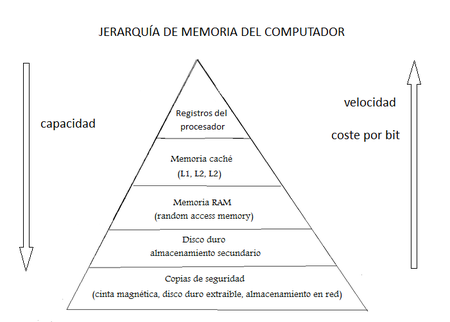
\includegraphics[width=8cm]{Jerarquia de la memoria.png}
\centering
\caption{Jerarquia memoria}
\label{fig:cpplogo}
\end{figure}

\subsection{¿Qué hace que una memoria sea más rápida que otra?}
4. ¿Qué hace que una memoria sea más rápida que otra? ¿Por qué esto es importante?\vspace{0.5cm}




Lo que hace más rapida una memoria que otra lo podemos ver de dos maneras, primero sus materiales de construcción los cuales pueden ser mejores conductores o mejores para retener  los datos que se le dan, y segundo por el modo en el que se guarda la información como por ejemplo el disco duro el cual tiene que girar un motor a gran velocidad para poder leer o escribir cualquier tipo de información lo que hace que el proceso tarde más, en cambio las unidades DRAM usan un proceso de almacenamiento por bits, estas se organizan de modo de celdas las cuales almacenan una pequeña parte de la información y al momento de acceder a ellas sólo es saber en qué posición está dicha información para ser usada, pero a pesar de ser rapida este proceso tiene el fallo de tener que estar alimentando sus terminales antes de que su información desaparezca por no tener suficiente energia en sus celdas, este problema lo resuelve la memoria cache la cual acúa de manera similar a la memoria DRAM solo que sin el problema de la corriente electrica constantemente ya que en su arquitectura se logra hacer que este paso no sea necesario, pero esta se usa en pequeña medida ya que su costo es elevado a comparación de las otras memorias.
\section{Conclusiónes}
Al terminar este trabajo de investigación me he dado cuenta que el sistema de memorias de un computador es como una composición de engranajes; los cuales necesitan siempre del otro para su correcta función, si falla alguno su función principal será interrumpida, todo este sistema de memorias ha sido posible gracias a que personas pensaron la forma más optima posible para llevar a cabo las tareas de los computadores, seguramente en unos años a este sistema se le añadiran mejoras las cuales harán de estos procesos algo mucho más rapido de lo que tenemos ahora, por lo pronto sólo queda dar un entendimiento de lo que significa todo esto para comprender de una mejor manera la funcionalidad de los computadores.
\bibliographystyle{IEEEtran}
\bibliography{references.bib}

\end{document}
